% =============================================================================
% DeSFAM Final Seminar Presentation
% Structure aligned with instructor requirements
% Cross-referenced against IEEE Access 2025 paper
% =============================================================================
\documentclass[aspectratio=169,11pt]{beamer}

\usepackage[utf8]{inputenc}
\usepackage[T1]{fontenc}
\usepackage{graphicx}
\usepackage{booktabs}
\usepackage{amsmath,amssymb}
\usepackage{tikz}
\usepackage[most]{tcolorbox}
\usetikzlibrary{shapes.geometric, arrows.meta, positioning, calc, fit, backgrounds, matrix}

%------------------------------------------------------------------------------
% COLOR PALETTE
%------------------------------------------------------------------------------
\definecolor{Navy}{RGB}{10,37,64}
\definecolor{Teal}{RGB}{0,150,140}
\definecolor{Gold}{RGB}{218,165,32}
\definecolor{SJCETblue}{RGB}{25, 55, 95}
\definecolor{SJCETgold}{RGB}{184, 134, 11}
\definecolor{DarkGray}{RGB}{80, 80, 80}
\definecolor{SoftRed}{RGB}{200,60,60}
\definecolor{LightBG}{RGB}{248,250,252}
\definecolor{TextGray}{RGB}{60,70,80}

%------------------------------------------------------------------------------
% BEAMER THEME SETUP
%------------------------------------------------------------------------------
\usetheme{default}
\setbeamercolor{background canvas}{bg=LightBG}
\setbeamercolor{normal text}{fg=TextGray}
\setbeamercolor{frametitle}{fg=Navy,bg=}
\setbeamercolor{title}{fg=Navy}
\setbeamercolor{subtitle}{fg=Teal}
\setbeamercolor{author}{fg=TextGray}
\setbeamercolor{institute}{fg=TextGray!70}
\setbeamercolor{date}{fg=TextGray!70}
\setbeamercolor{item}{fg=Teal}
\setbeamercolor{block title}{fg=white,bg=Navy}
\setbeamercolor{block body}{fg=TextGray,bg=Navy!8}
\setbeamercolor{block title example}{fg=white,bg=Teal}
\setbeamercolor{block body example}{fg=TextGray,bg=Teal!8}
\setbeamercolor{block title alerted}{fg=white,bg=SoftRed}
\setbeamercolor{block body alerted}{fg=TextGray,bg=SoftRed!8}

\setbeamerfont{frametitle}{size=\LARGE,series=\bfseries}
\setbeamerfont{title}{size=\Huge,series=\bfseries}
\setbeamerfont{subtitle}{size=\large}
\setbeamertemplate{navigation symbols}{}
\setbeamertemplate{footline}[frame number]
\setbeamertemplate{itemize items}[circle]

\setbeamertemplate{frametitle}{
  \vspace{0.4cm}
  {\usebeamerfont{frametitle}\insertframetitle\par}
  \vspace{-0.15cm}
  {\color{Teal}\rule{\textwidth}{1.5pt}}
  \vspace{0.25cm}
}

%------------------------------------------------------------------------------
% Footer: Solid SJCETblue bar, white text, full college name
%------------------------------------------------------------------------------
\setbeamercolor{author in head/foot}{bg=SJCETblue,fg=white}
\setbeamercolor{date in head/foot}{bg=SJCETblue,fg=white}

\setbeamertemplate{footline}{%
  \leavevmode%
  \hbox{%
    \begin{beamercolorbox}[wd=.80\paperwidth,ht=3.4ex,dp=1.3ex,leftskip=0.5cm,colsep=0pt]{author in head/foot}%
      \usebeamerfont{author in head/foot}%
      \small St. Joseph's College of Engineering and Technology, Palai%
    \end{beamercolorbox}%
    \begin{beamercolorbox}[wd=.20\paperwidth,ht=3.4ex,dp=1.3ex,rightskip=0.5cm,colsep=0pt]{date in head/foot}%
      \usebeamerfont{date in head/foot}%
      \raggedleft\small\textbf{\insertframenumber{} / \inserttotalframenumber}%
    \end{beamercolorbox}%
  }%
}


%------------------------------------------------------------------------------
% CUSTOM COMMANDS & TIKZ STYLES
%------------------------------------------------------------------------------
\newcommand{\cmark}{{\color{Teal}\checkmark}}
\newcommand{\xmark}{{\color{SoftRed}$\times$}}
\newcommand{\pmark}{{\color{Gold!80!black}$\sim$}}

\tikzset{
  card/.style={draw=Navy, rounded corners=4pt, fill=white, thick,
    minimum width=2.6cm, minimum height=1.1cm, align=center, font=\small},
  phasebox/.style={draw=Teal, line width=1.5pt, rounded corners=6pt, fill=white, thick,
    minimum width=2.8cm, minimum height=1.6cm, align=center, text width=2.4cm, font=\small},
  arrowflow/.style={-{Stealth[length=3mm]}, line width=2pt, Teal},
  iconnode/.style={circle, draw=Teal, fill=Teal!15, minimum size=1cm, font=\bfseries\small},
  bigstat/.style={font=\Huge\bfseries, color=Teal},
}

%------------------------------------------------------------------------------
% META INFORMATION
%------------------------------------------------------------------------------
\title[DeSFAM]{DeSFAM}
\subtitle{An Adaptive eBPF and AI-Driven Framework for Securing Cloud Containers in Real Time}
\author[Robert Thomas]{\textbf{Robert Thomas} \quad SJC23CC062}
\institute[SJCET]{Department of CSE (Cyber Security)\\St. Joseph's College of Engineering and Technology, Palai}
\date{August 2026}
\titlegraphic{}

\begin{document}

%------------------------------------------------------------------------------
% TITLE PAGE  (FIXED: date visible, tighter spacing, no center env padding)
%------------------------------------------------------------------------------
{
\setbeamertemplate{footline}{}
\setbeamertemplate{headline}{}
\begin{frame}[plain]

\vfill
\centering

\includegraphics[width=1.8cm]{sjcet_logo.png}

\vspace{0.2cm}
{\LARGE\bfseries\textcolor{SJCETblue}{DeSFAM}}\\[0.05cm]
{\large An Adaptive eBPF and AI-Driven Framework for\\[0.03cm]
Securing Cloud Containers in Real Time}

\vspace{0.15cm}
{\normalsize\textcolor{SJCETgold}{Final Seminar Presentation}}

\vspace{0.2cm}
\rule{0.45\textwidth}{0.5pt}

\vspace{0.2cm}
{\large Robert Thomas}\\[0.03cm]
{\normalsize SJC23CC062}

\vspace{0.15cm}
{\normalsize \textbf{Guide:} Prof. Aiswarya Mohan K}

\vspace{0.1cm}
{\small Department of Computer Science \& Engineering (Cyber Security)}\\[0.02cm]
{\small St. Joseph's College of Engineering and Technology, Palai}

\vspace{0.2cm}
{\normalsize August 2026}

\vfill

\end{frame}
}

%==============================================================================
% 2. INTRODUCTION
%==============================================================================
\begin{frame}{Introduction}
\begin{columns}[T]
\begin{column}{0.55\textwidth}
\textbf{Containerization} has transformed cloud deployment:
\begin{itemize}
  \item Lightweight, scalable, and portable
  \item Shared host kernel $\rightarrow$ low overhead
  \item Ideal for microservices and CI/CD pipelines
\end{itemize}

\vspace{0.3cm}
\textbf{The Hidden Risk:}
\begin{itemize}
  \item Containers share the \textbf{host OS kernel}
  \item \textbf{414 syscalls} exposed by default in Docker
  \item An attacker needs only \textbf{3--4 syscalls} to escape
\end{itemize}
\end{column}
\begin{column}{0.42\textwidth}
\centering
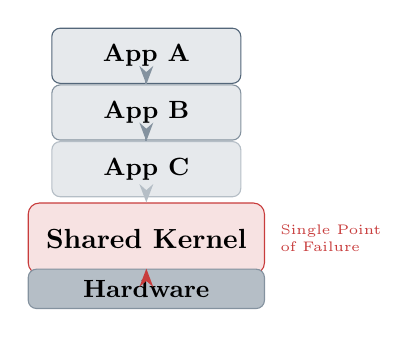
\begin{tikzpicture}[scale=0.8, every node/.style={font=\small}]
  \node[draw=Navy!70, fill=Navy!10, rounded corners=3pt, minimum width=2.4cm, minimum height=0.7cm, font=\small\bfseries] (app1) at (0,1.8) {App A};
  \node[draw=Navy!50, fill=Navy!10, rounded corners=3pt, minimum width=2.4cm, minimum height=0.7cm, font=\small\bfseries] (app2) at (0,0.9) {App B};
  \node[draw=Navy!30, fill=Navy!10, rounded corners=3pt, minimum width=2.4cm, minimum height=0.7cm, font=\small\bfseries] (app3) at (0,0) {App C};
  
  \node[draw=SoftRed, fill=SoftRed!15, rounded corners=4pt, minimum width=3cm, minimum height=0.9cm, font=\bfseries] (kernel) at (0,-1.1) {Shared Kernel};
  \node[draw=Navy!50, fill=Navy!30, rounded corners=3pt, minimum width=3cm, minimum height=0.5cm, font=\small\bfseries] (hw) at (0,-1.9) {Hardware};
  
  \draw[-{Stealth}, thick, Navy!50] (app1) -- (app2);
  \draw[-{Stealth}, thick, Navy!50] (app2) -- (app3);
  \draw[-{Stealth}, thick, Navy!30] (app3) -- (kernel);
  \draw[-{Stealth}, thick, SoftRed] (kernel) -- (hw);
  
  \node[right=0.3cm, font=\tiny, align=left, SoftRed] at (1.6,-1.1) {Single Point\\of Failure};
\end{tikzpicture}
\end{column}
\end{columns}

\vspace{0.3cm}
\begin{exampleblock}{What is DeSFAM?}
\textbf{D}ynamic \textbf{e}BPF-driven \textbf{S}yscall \textbf{F}iltering and \textbf{A}nomaly \textbf{M}itigation --- a real-time framework that shrinks the attack surface and blocks exploits in \textbf{under 1 ms}.
\end{exampleblock}
\end{frame}

%==============================================================================
% 3. PROBLEM STATEMENT
%==============================================================================
\begin{frame}{Problem Statement}
\centering
\begin{tikzpicture}[
  gapbox/.style={draw, rounded corners=5pt, fill=white, thick, 
    minimum width=3.2cm, minimum height=1.3cm, align=center, font=\small,
    blur shadow={shadow blur steps=5, shadow xshift=1pt, shadow yshift=-1pt, shadow opacity=10}}
]
  \node[gapbox, draw=SoftRed, fill=SoftRed!8] (g1) at (0,0) 
    {{\color{SoftRed}\textbf{Over-Permissive}}\\[1pt]\tiny 414 default syscalls};
  \node[gapbox, draw=Gold, fill=Gold!10, right=0.6cm of g1] (g2) 
    {{\color{Gold!80!black}\textbf{Static Policies}}\\[1pt]\tiny No runtime adaptation};
  \node[gapbox, draw=Navy, fill=Navy!8, below=0.5cm of g1] (g3) 
    {{\color{Navy}\textbf{Blind to Sequences}}\\[1pt]\tiny Single-call filtering only};
  \node[gapbox, draw=Teal, fill=Teal!8, right=0.6cm of g3] (g4) 
    {{\color{Teal}\textbf{Slow Enforcement}}\\[1pt]\tiny User-space latency};

  \draw[dashed, gray, thick] ($(g1.north west)+(-0.3,0.3)$) rectangle ($(g4.south east)+(0.3,-0.3)$);
  \node[fill=LightBG, font=\small\bfseries, text=Navy] at ($(g1.north)!0.5!(g2.north)+(0,0.45)$) {Four Critical Gaps};
\end{tikzpicture}

\vspace{0.4cm}
{\normalsize\bfseries\textcolor{Navy}{Research Question}\\[4pt]}
\boxed{\textit{How do we shrink the attack surface and stop exploits in real time---without breaking anything?}}
\end{frame}

%==============================================================================
% 4. OBJECTIVES
%==============================================================================
\begin{frame}{Objectives}
\centering
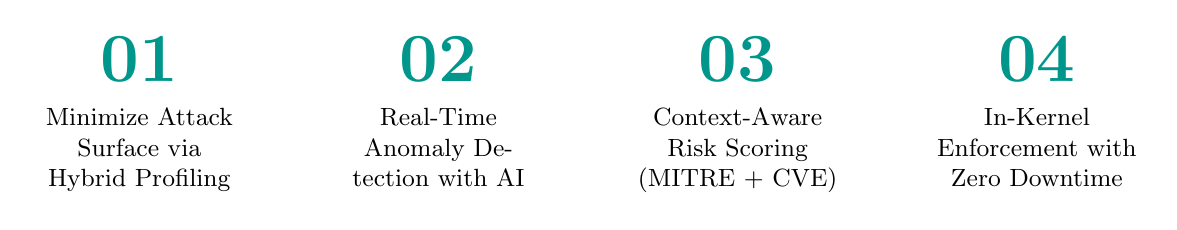
\begin{tikzpicture}[node distance=0.1cm]
  \node[bigstat] (n1) at (0,0) {01};
  \node[below=0.1cm of n1, align=center, font=\small, text width=2.6cm] {Minimize Attack Surface via Hybrid Profiling};

  \node[bigstat] (n2) at (3.8,0) {02};
  \node[below=0.1cm of n2, align=center, font=\small, text width=2.6cm] {Real-Time Anomaly Detection with AI};

  \node[bigstat] (n3) at (7.6,0) {03};
  \node[below=0.1cm of n3, align=center, font=\small, text width=2.6cm] {Context-Aware Risk Scoring (MITRE + CVE)};

  \node[bigstat] (n4) at (11.4,0) {04};
  \node[below=0.1cm of n4, align=center, font=\small, text width=2.6cm] {In-Kernel Enforcement with Zero Downtime};
\end{tikzpicture}
\end{frame}

%==============================================================================
% 5. LITERATURE SURVEY
%==============================================================================
\begin{frame}{Literature Survey}
\centering
\footnotesize
\begin{tabular}{@{}llcc@{}}
\toprule
\textbf{Paper} & \textbf{Core Technique} & \textbf{Year} & \textbf{Venue} \\
\midrule
\textbf{DeSFAM} & Hybrid + VAE/iForest + eBPF/LSM & 2025 & IEEE Access \\
Confine & Static call-graph $\rightarrow$ seccomp & 2023 & Computers \& Security \\
Prof-gen & Boot-time trace + static check & 2021 & IEEE CLOUD \\
Optimus & Association-rule mining on eBPF & 2024 & J. Cloud Computing \\
KubeRosy & eBPF + Kubernetes CRD updates & 2024 & IEEE Access \\
PACED & Provenance graph tracking & 2022 & IEEE IC2E \\
Condo & Hardware TEE for kernel data & 2024 & IEEE TIFS \\
\bottomrule
\end{tabular}

\vspace{0.4cm}
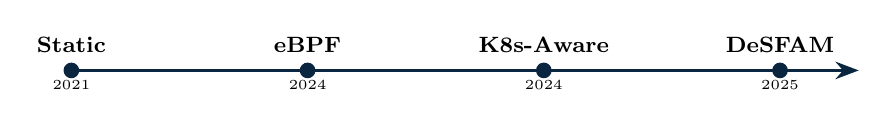
\begin{tikzpicture}
  \draw[-{Stealth}, very thick, Navy] (0,0) -- (10,0);
  \foreach \x/\y/\t in {0/2021/Static, 3/2024/eBPF, 6/2024/K8s-Aware, 9/2025/\textbf{DeSFAM}} {
    \node[circle, fill=Navy, inner sep=2pt, label={above:{\footnotesize\bfseries\t}}] at (\x,0) {};
    \node[below, font=\tiny] at (\x,0) {\y};
  }
\end{tikzpicture}
\end{frame}

%==============================================================================
% 6. COMPARATIVE ANALYSIS
%==============================================================================
\begin{frame}{Comparative Analysis}
\centering
\resizebox{0.98\textwidth}{!}{%
\begin{tabular}{@{}lccccccc@{}}
\toprule
 & \textbf{Conf.} & \textbf{Prof} & \textbf{NIMOS} & \textbf{Opt.} & \textbf{K8sR} & \textbf{Condo} & \cellcolor{Teal!15}\textbf{DeSFAM} \\
\midrule
Hybrid Profiling & \cmark & \cmark & \cmark & \xmark & \xmark & \xmark & \cellcolor{Teal!15}\cmark \\
Live eBPF & \xmark & \xmark & \xmark & \cmark & \cmark & \xmark & \cellcolor{Teal!15}\cmark \\
AI Detection & \xmark & \xmark & \xmark & \xmark & \xmark & \xmark & \cellcolor{Teal!15}\cmark \\
In-Kernel Block & \xmark & \xmark & \xmark & \pmark & \cmark & \xmark & \cellcolor{Teal!15}\cmark \\
Auto-Hardening & \xmark & \xmark & \xmark & \pmark & \cmark & \xmark & \cellcolor{Teal!15}\cmark \\
Zero Restart & \xmark & \xmark & \xmark & \xmark & \cmark & \xmark & \cellcolor{Teal!15}\cmark \\
Real-Time CVE Blocking & Static & Hybrid & \xmark & Observed & Predefined & \xmark & \cellcolor{Teal!15}\cmark \\
\midrule
\textbf{SRR (\%)} & 47.6 & 67.8 & 63.4 & 57.1 & 45.3 & --- & \cellcolor{Teal!15}\textbf{78.6} \\
\bottomrule
\end{tabular}%
}

\vspace{0.3cm}

\begin{tikzpicture}
  \node[fill=Teal, text=white, rounded corners=3pt, inner sep=6pt, font=\bfseries\small] {
    Only framework covering all layers: Profile $\cdot$ Detect $\cdot$ Enforce $\cdot$ Adapt
  };
\end{tikzpicture}
\end{frame}

%==============================================================================
% SECTION: DETAILED EXPLANATION OF MAIN PAPER
%==============================================================================
\section{Detailed Explanation of the Selected Main Paper}

%==============================================================================
% 7. BACKGROUND & MOTIVATION
%==============================================================================
\begin{frame}{Background \& Motivation}
\begin{columns}[T]
\begin{column}{0.48\textwidth}
\textbf{Container Security Foundations}
\begin{itemize}
  \item Containers use \textbf{namespaces} and \textbf{cgroups} for isolation
  \item But the \textbf{kernel is shared} across all containers
  \item \textbf{Syscalls} are the primary gateway for attacks
\end{itemize}

\vspace{0.2cm}
\textbf{Existing Defenses}
\begin{itemize}
  \item \textbf{Seccomp-BPF}: Standard but static and coarse
  \item \textbf{AppArmor/SELinux}: Rule-based, manual upkeep
  \item None adapt to runtime behavior or detect sequences
\end{itemize}
\end{column}
\begin{column}{0.48\textwidth}
\begin{exampleblock}{Key Insight}
A simple nginx container has access to \textbf{414 syscalls}. An attacker needs only \textbf{3--4} to escape.
\end{exampleblock}

\vspace{0.15cm}
\begin{block}{The Evolution}
\centering
Static Profiles $\longrightarrow$ Dynamic eBPF $\longrightarrow$ \textbf{DeSFAM}\\[2pt]
{\small AI + eBPF + Self-Healing}
\end{block}
\end{column}
\end{columns}
\end{frame}

%==============================================================================
% 8. PROBLEM ADDRESSED
%==============================================================================
\begin{frame}{Problem Addressed}
\centering
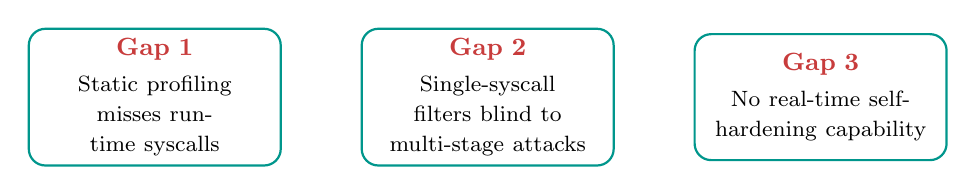
\begin{tikzpicture}[node distance=1cm]
  \node[phasebox, minimum width=3.2cm, text width=2.8cm] (g1) 
    {{\color{SoftRed}\textbf{Gap 1}}\\[2pt]\footnotesize Static profiling misses runtime syscalls};
  \node[phasebox, minimum width=3.2cm, text width=2.8cm, right=of g1] (g2) 
    {{\color{SoftRed}\textbf{Gap 2}}\\[2pt]\footnotesize Single-syscall filters blind to multi-stage attacks};
  \node[phasebox, minimum width=3.2cm, text width=2.8cm, right=of g2] (g3) 
    {{\color{SoftRed}\textbf{Gap 3}}\\[2pt]\footnotesize No real-time self-hardening capability};
\end{tikzpicture}

\vspace{0.5cm}
\begin{exampleblock}{DeSFAM's Answer}
Unify \textbf{minimal exposure} (Phase 1), \textbf{sequence-aware detection} (Phase 2), and \textbf{sub-millisecond in-kernel enforcement} (Phase 3) --- all without container restarts.
\end{exampleblock}
\end{frame}

%==============================================================================
% 9. PROPOSED METHODOLOGY
%==============================================================================
\begin{frame}{Proposed Methodology: 3-Phase Pipeline}
\centering
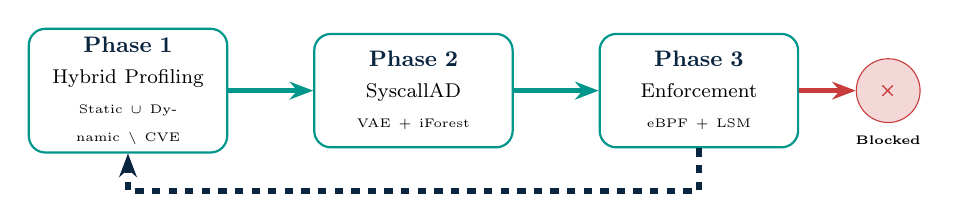
\begin{tikzpicture}[node distance=1.2cm, scale=0.9, transform shape]
  \node[phasebox, minimum width=2.8cm, text width=2.4cm] (ph1)
    {{\color{Navy}\textbf{Phase 1}}\\[3pt]\footnotesize Hybrid Profiling\\[1pt]\tiny Static $\cup$ Dynamic $\setminus$ CVE};
  \node[phasebox, minimum width=2.8cm, text width=2.4cm, right=of ph1] (ph2)
    {{\color{Navy}\textbf{Phase 2}}\\[3pt]\footnotesize SyscallAD\\[1pt]\tiny VAE + iForest};
  \node[phasebox, minimum width=2.8cm, text width=2.4cm, right=of ph2] (ph3)
    {{\color{Navy}\textbf{Phase 3}}\\[3pt]\footnotesize Enforcement\\[1pt]\tiny eBPF + LSM};

  \draw[arrowflow] (ph1) -- (ph2);
  \draw[arrowflow] (ph2) -- (ph3);
  \draw[arrowflow, dashed, Navy] (ph3.south) -- ++(0,-0.6) -| (ph1.south);

  \node[right=0.8cm of ph3, iconnode, fill=SoftRed!20, draw=SoftRed, minimum size=0.9cm] (out)
    {{\color{SoftRed}\scriptsize\bfseries \texttimes}};
  \node[below=0.05cm of out, font=\tiny\bfseries] {Blocked};
  \draw[arrowflow, SoftRed] (ph3) -- (out);
\end{tikzpicture}

\vspace{0.3cm}
{\small\textcolor{TextGray}{Feedback loop auto-hardens policies without container restarts.}}
\end{frame}

%==============================================================================
% 10. SYSTEM ARCHITECTURE
%==============================================================================
\begin{frame}{System Architecture}
\centering
\includegraphics[width=0.85\textwidth,height=0.60\textheight,keepaspectratio]{fig1_architecture.png}
\vspace{0.15cm}

{\small\textcolor{TextGray}{User-space profiling $\rightarrow$ AI detection $\rightarrow$ Kernel-space eBPF enforcement}}
\end{frame}

%==============================================================================
% 11. ALGORITHMS & TECHNOLOGIES
%==============================================================================
\begin{frame}{Algorithms \& Technologies}
\begin{columns}[T]
\begin{column}{0.48\textwidth}
\textbf{Core Technologies}
\begin{itemize}
  \item \textbf{eBPF / bcc} --- Kernel instrumentation
  \item \textbf{LSM Hooks} --- Kernel enforcement layer
  \item \textbf{VAE + iForest} --- Deep + Statistical ML
  \item \textbf{PrefixSpan} --- Frequent pattern mining
  \item \textbf{NVD API + NLP} --- Threat intelligence
\end{itemize}
\end{column}
\begin{column}{0.48\textwidth}
\textbf{Key Algorithms}
\begin{enumerate}
  \item Hybrid Syscall Profiling (Phase 1)
  \item Real-Time Anomaly Detection (Phase 2)
  \item Adaptive Enforcement + Auto-Hardening (Phase 3)
\end{enumerate}

\vspace{0.15cm}
\begin{block}{Ensemble Fusion Formula}
\footnotesize
\vspace{-0.2cm}
\[
A(W_i) = 0.7\,A_{\text{VAE}} + 0.3\,A_{\text{iForest}}
\]
\vspace{-0.2cm}
{\tiny $\alpha = 0.7$ validated via sensitivity analysis on DongTing dataset}
\end{block}
\end{column}
\end{columns}
\end{frame}

%==============================================================================
% 12. PHASE 1: HYBRID PROFILING
%==============================================================================
\begin{frame}{Phase 1: Hybrid Syscall Profiling}
\centering
\includegraphics[width=0.82\textwidth,height=0.50\textheight,keepaspectratio]{fig2_phase1.png}
\vspace{0.15cm}

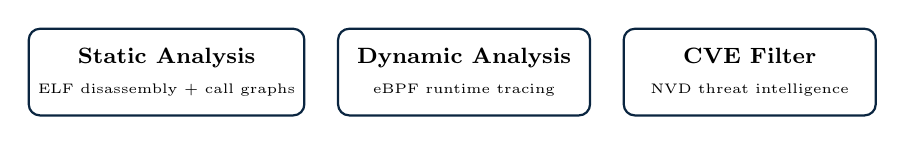
\begin{tikzpicture}[node distance=0.4cm]
  \node[card, minimum width=3.2cm] (s1) {\footnotesize\textbf{Static Analysis}\\\tiny ELF disassembly + call graphs};
  \node[card, minimum width=3.2cm, right=of s1] (s2) {\footnotesize\textbf{Dynamic Analysis}\\\tiny eBPF runtime tracing};
  \node[card, minimum width=3.2cm, right=of s2] (s3) {\footnotesize\textbf{CVE Filter}\\\tiny NVD threat intelligence};
\end{tikzpicture}

\vspace{0.2cm}
{\footnotesize Final list: $S_{\text{final}} = \big((S_{\text{static}} \cup S_{\text{dynamic}}) \cap S_{\text{template}}\big) \setminus \big(S_{\text{blocked}} \setminus S_{\text{template}}\big)$}
\end{frame}

%==============================================================================
% 13. PHASE 2: SYSCALLAD
%==============================================================================
\begin{frame}{Phase 2: SyscallAD --- AI Anomaly Detection}
\begin{columns}[T]
\begin{column}{0.48\textwidth}
\centering
\includegraphics[width=\textwidth,height=0.50\textheight,keepaspectratio]{fig4_phase2.png}
\end{column}
\begin{column}{0.48\textwidth}
\begin{block}{How It Works}
\begin{itemize}
  \item \textbf{VAE} learns ``normal'' per-container behavior
  \item \textbf{iForest} spots statistical outliers
  \item \textbf{Ensemble} fuses both scores ($\alpha = 0.7$)
  \item \textbf{Dynamic EMA threshold} adapts to drift
\end{itemize}
\end{block}

\vspace{0.1cm}
\begin{alertblock}{Training Data}
\footnotesize
DongTing dataset: \textbf{18,966} syscall sequences\\
6,850 benign + 12,116 malicious sequences
\end{alertblock}
\end{column}
\end{columns}
\end{frame}

%==============================================================================
% 14. PHASE 3: ENFORCEMENT
%==============================================================================
\begin{frame}{Phase 3: Adaptive Enforcement}
\centering
\includegraphics[width=0.78\textwidth,height=0.48\textheight,keepaspectratio]{fig8_phase3.png}
\vspace{0.15cm}

\begin{columns}[T]
\begin{column}{0.32\textwidth}
\centering
\textbf{Risk $<$ 5}\\Log Only
\end{column}
\begin{column}{0.32\textwidth}
\centering
\textbf{Risk 5--8}\\Rate-Limit
\end{column}
\begin{column}{0.32\textwidth}
\centering
\textbf{Risk $\geq$ 8}\\Block via LSM
\end{column}
\end{columns}

\vspace{0.2cm}
{\footnotesize Risk Score = $\sum$ Severity(t) + 5 $\cdot$ $\mathbb{I}$(Exploit Match)}
\end{frame}

%==============================================================================
% 15. DETAILED WORKING
%==============================================================================
\begin{frame}{Detailed Working: Stopping a Real Attack}
\centering
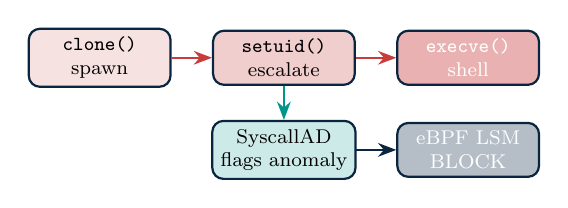
\begin{tikzpicture}[scale=0.9, transform shape]
  \node[card, fill=SoftRed!15, minimum width=2cm, minimum height=0.7cm, font=\footnotesize] (s1) at (0,0) {\texttt{clone()}\\spawn};
  \node[card, fill=SoftRed!25, minimum width=2cm, minimum height=0.7cm, font=\footnotesize] (s2) at (2.6,0) {\texttt{setuid()}\\escalate};
  \node[card, fill=SoftRed!40, text=white, minimum width=2cm, minimum height=0.7cm, font=\footnotesize] (s3) at (5.2,0) {\texttt{execve()}\\shell};
  
  \node[card, fill=Teal!20, minimum width=2cm, minimum height=0.7cm, font=\footnotesize] (d1) at (2.6,-1.3) {SyscallAD\\flags anomaly};
  \node[card, fill=Navy!30, text=white, minimum width=2cm, minimum height=0.7cm, font=\footnotesize] (d2) at (5.2,-1.3) {eBPF LSM\\BLOCK};
  
  \draw[-{Stealth}, thick, SoftRed] (s1) -- (s2);
  \draw[-{Stealth}, thick, SoftRed] (s2) -- (s3);
  \draw[-{Stealth}, thick, Teal] (s2) -- (d1);
  \draw[-{Stealth}, thick, Navy] (d1) -- (d2);
\end{tikzpicture}

\vspace{0.3cm}
\begin{columns}[T]
\begin{column}{0.30\textwidth}
\centering
\textbf{1. Detect}\\AI spots unusual \texttt{setuid} in context
\end{column}
\begin{column}{0.30\textwidth}
\centering
\textbf{2. Decide}\\Risk score $\geq$ 8 triggers block
\end{column}
\begin{column}{0.30\textwidth}
\centering
\textbf{3. Enforce}\\Kernel denial in \textbf{0.54 $\mu$s}
\end{column}
\end{columns}
\end{frame}

%==============================================================================
% 16. EXPERIMENTAL SETUP
%==============================================================================
\begin{frame}{Experimental Setup}
\begin{columns}[T]
\begin{column}{0.48\textwidth}
\begin{block}{Infrastructure}
\begin{itemize}
  \item Ubuntu 24.04 LTS, 16-core CPU, 64 GB RAM
  \item NVIDIA A100 (for model training)
\end{itemize}
\end{block}
\begin{block}{Workloads Tested}
\begin{itemize}
  \item Nginx, MySQL, Redis, Node.js, Python, MongoDB
\end{itemize}
\end{block}
\end{column}
\begin{column}{0.48\textwidth}
\begin{alertblock}{Attack Simulation (14 CVEs)}
\footnotesize
CVE-2021-4034 (Polkit), CVE-2022-0847 (Dirty Pipe), CVE-2019-5736 (runc), CVE-2021-22555, CVE-2022-0185, \textit{et al.}
\end{alertblock}
\begin{exampleblock}{Baselines Compared}
Confine, Prof-gen, NIMOS, Optimus, KubeRosy
\end{exampleblock}
\end{column}
\end{columns}
\end{frame}

%==============================================================================
% 17. RESULTS: SYSCALL REDUCTION
%==============================================================================
\begin{frame}{Results: Syscall Reduction}
\centering
\includegraphics[width=0.70\textwidth,height=0.55\textheight,keepaspectratio]{fig9_srr.png}
\vspace{0.15cm}

\textbf{78.6\% SRR} --- Down from 414 (Docker default) to $\sim$89 syscalls.\\
{\footnotesize Smallest whitelist among all baselines (Table 6)}
\end{frame}

%==============================================================================
% 18. RESULTS: PERFORMANCE OVERHEAD
%==============================================================================
\begin{frame}{Results: Performance Overhead}
\begin{columns}[T]
\begin{column}{0.48\textwidth}
\centering
\includegraphics[width=\textwidth,height=0.45\textheight,keepaspectratio]{fig11_cpu.png}
\vspace{0.05cm}

{\small CPU Overhead: \textbf{+1.74\%}}
\end{column}
\begin{column}{0.48\textwidth}
\centering
\includegraphics[width=\textwidth,height=0.45\textheight,keepaspectratio]{fig12_memory.png}
\vspace{0.05cm}

{\small Memory: \textbf{--6.1\%} (saved via blocked exploits)}
\end{column}
\end{columns}

\vspace{0.2cm}
\centering
\textbf{Policy updates: $<$100$\mu$s with zero downtime}
\end{frame}

%==============================================================================
% 19. RESULTS: DETECTION & BLOCKING
%==============================================================================
\begin{frame}{Results: Detection Accuracy \& CVE Blocking}
\begin{columns}[T]
\begin{column}{0.48\textwidth}
\begin{block}{SyscallAD Performance}
\footnotesize
\begin{tabular}{@{}lccc@{}}
\toprule
\textbf{Class} & \textbf{Precision} & \textbf{Recall} & \textbf{F1} \\
\midrule
Normal & 0.97 & 0.98 & 0.97 \\
Attack & 0.94 & 0.90 & 0.92 \\
\midrule
\multicolumn{4}{l}{\textbf{Accuracy: 96\%} $\quad$ \textbf{AUC: 0.94}} \\
\bottomrule
\end{tabular}
\end{block}
\vspace{0.1cm}
\begin{alertblock}{False Positive Rate}
\textbf{1.6\%} --- Lowest among all baselines
\end{alertblock}
\end{column}
\begin{column}{0.48\textwidth}
\begin{exampleblock}{CVE Blocking Summary}
\footnotesize
\begin{itemize}
  \item \textbf{14/14} real-world attack scenarios blocked
  \item \textbf{0.540 $\mu$s} enforcement latency
  \item \textbf{1.82 ms} average detection latency
  \item All baselines missed $\geq$ 3 attacks each
\end{itemize}
\end{exampleblock}
\end{column}
\end{columns}
\end{frame}

%==============================================================================
% 20. KEY FINDINGS & CONTRIBUTIONS
%==============================================================================
\begin{frame}{Key Findings \& Contributions}
\begin{columns}[T]
\begin{column}{0.48\textwidth}
\textbf{Key Findings}
\begin{itemize}
  \item Hybrid profiling captures expected + runtime syscalls
  \item VAE+iForest needs \textbf{no retraining} for zero-days
  \item Dynamic EMA threshold suppresses false positives
  \item In-kernel enforcement is \textbf{3--65$\times$ faster} than user-space
\end{itemize}
\end{column}
\begin{column}{0.48\textwidth}
\textbf{Contributions}
\begin{enumerate}
  \item Hybrid profiling pipeline (static + dynamic + CVE)
  \item SyscallAD (VAE + iForest ensemble)
  \item MITRE + CVE contextual risk scoring
  \item Fine-grained eBPF/LSM enforcement
  \item Runtime auto-hardening feedback loop
\end{enumerate}
\end{column}
\end{columns}
\end{frame}

%==============================================================================
% 21. ADVANTAGES
%==============================================================================
\begin{frame}{Advantages}
\centering
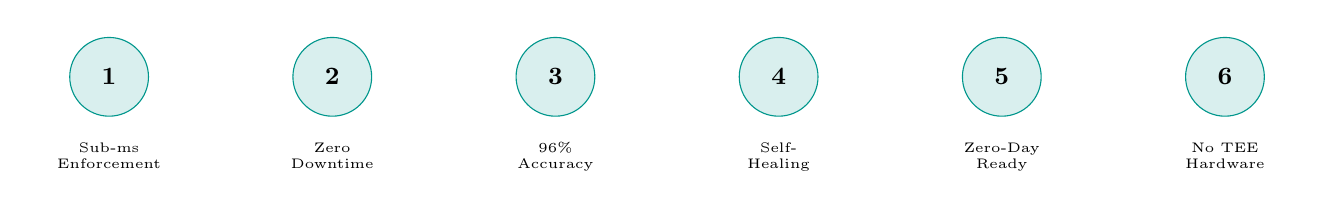
\begin{tikzpicture}
\matrix[matrix of nodes, column sep=1cm, row sep=0.2cm, ampersand replacement=\&,
        nodes={align=center, font=\small}] {
  \node[iconnode] {1}; \& \node[iconnode] {2}; \& \node[iconnode] {3}; \&
  \node[iconnode] {4}; \& \node[iconnode] {5}; \& \node[iconnode] {6}; \\
  \node[text width=1.6cm, font=\tiny] {Sub-ms\\Enforcement}; \&
  \node[text width=1.6cm, font=\tiny] {Zero\\Downtime}; \&
  \node[text width=1.6cm, font=\tiny] {96\%\\Accuracy}; \&
  \node[text width=1.6cm, font=\tiny] {Self-\\Healing}; \&
  \node[text width=1.6cm, font=\tiny] {Zero-Day\\Ready}; \&
  \node[text width=1.6cm, font=\tiny] {No TEE\\Hardware}; \\
};
\end{tikzpicture}

\vspace{0.3cm}
\begin{columns}[T]
\begin{column}{0.48\textwidth}
\begin{itemize}
  \item \textbf{Smallest whitelist} (89 syscalls) vs. 414 default
  \item \textbf{Lowest FPR} (1.6\%) among all compared frameworks
  \item \textbf{No container restarts} for policy updates
\end{itemize}
\end{column}
\begin{column}{0.48\textwidth}
\begin{itemize}
  \item \textbf{Retraining-free} anomaly detection
  \item \textbf{Context-aware} blocking via MITRE + CVE
  \item \textbf{Portable}: Pure software, no hardware dependency
\end{itemize}
\end{column}
\end{columns}
\end{frame}

%==============================================================================
% 22. APPLICATIONS
%==============================================================================
\begin{frame}{Applications}
\centering
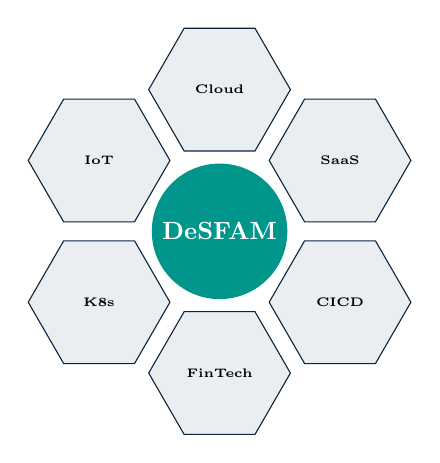
\begin{tikzpicture}[scale=0.9, transform shape]
  \foreach \a/\t/\x/\y in {
    0/Cloud/0/2,
    60/SaaS/1.7/1,
    120/CI\/CD/1.7/-1,
    180/FinTech/0/-2,
    240/K8s/-1.7/-1,
    300/IoT/-1.7/1
  } {
    \node[regular polygon, regular polygon sides=6, draw=Navy, fill=Navy!8,
          minimum size=2cm, align=center, font=\tiny\bfseries] at (\x,\y) {\t};
  }
  \node[circle, fill=Teal, text=white, minimum size=1.2cm, font=\bfseries] at (0,0) {DeSFAM};
\end{tikzpicture}

\vspace{0.3cm}
{\small Any multi-tenant container environment requiring real-time, adaptive syscall security}
\end{frame}

%==============================================================================
% 23. LIMITATIONS
%==============================================================================
\begin{frame}{Limitations}
\centering
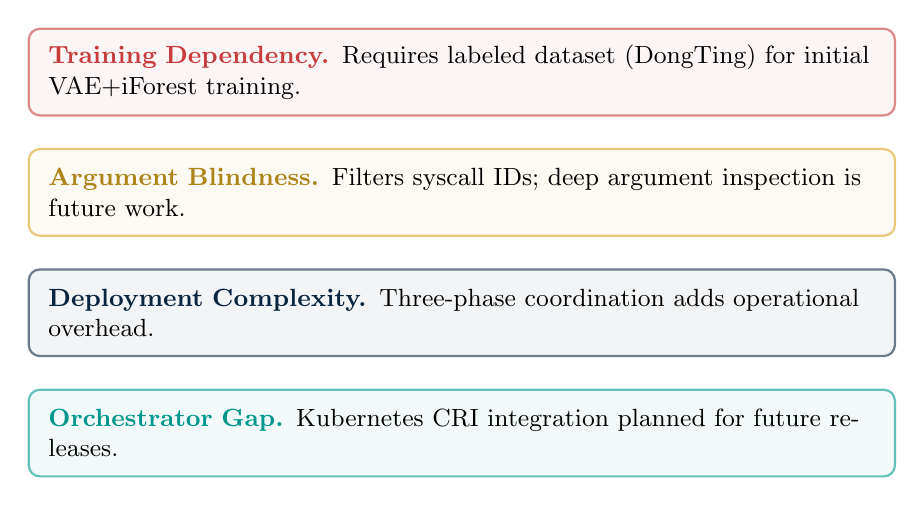
\begin{tikzpicture}[node distance=0.4cm]
  \node[card, minimum width=11cm, text width=10.5cm, align=left, fill=SoftRed!5, draw=SoftRed!60] (l1)
    {{\bfseries\color{SoftRed}Training Dependency.} Requires labeled dataset (DongTing) for initial VAE+iForest training.};
  \node[card, minimum width=11cm, text width=10.5cm, align=left, below=of l1, fill=Gold!5, draw=Gold!60] (l2)
    {{\bfseries\color{Gold!80!black}Argument Blindness.} Filters syscall IDs; deep argument inspection is future work.};
  \node[card, minimum width=11cm, text width=10.5cm, align=left, below=of l2, fill=Navy!5, draw=Navy!60] (l3)
    {{\bfseries\color{Navy}Deployment Complexity.} Three-phase coordination adds operational overhead.};
  \node[card, minimum width=11cm, text width=10.5cm, align=left, below=of l3, fill=Teal!5, draw=Teal!60] (l4)
    {{\bfseries\color{Teal}Orchestrator Gap.} Kubernetes CRI integration planned for future releases.};
\end{tikzpicture}
\end{frame}

%==============================================================================
% 24. CONCLUSION
%==============================================================================
\begin{frame}{Conclusion}
\begin{columns}[T]
\begin{column}{0.22\textwidth}
\begin{block}{\centering 78.6\%}
\centering Syscall\\Reduction
\end{block}
\end{column}
\begin{column}{0.22\textwidth}
\begin{block}{\centering 96\%}
\centering Detection\\Accuracy
\end{column}
\end{column}
\begin{column}{0.22\textwidth}
\begin{block}{\centering 0.54$\mu$s}
\centering Enforcement\\Latency
\end{column}
\end{column}
\begin{column}{0.22\textwidth}
\begin{block}{\centering 14/14}
\centering CVEs\\Blocked
\end{block}
\end{column}
\end{columns}

\vspace{0.3cm}
\begin{exampleblock}{Key Takeaways}
\begin{itemize}
  \item \textbf{Hybrid Profiling} minimizes attack surface without breaking functionality
  \item \textbf{SyscallAD} detects zero-day sequence attacks with high precision
  \item \textbf{eBPF LSM Enforcement} provides sub-millisecond, in-kernel blocking
  \item \textbf{Self-healing policies} auto-harden over time with zero downtime
\end{itemize}
\end{exampleblock}
\end{frame}

%==============================================================================
% 25. REFERENCES
%==============================================================================
\begin{frame}{References}
\footnotesize
\begin{enumerate}
  \item S. Zehra \textit{et al.}, ``DeSFAM: An Adaptive eBPF and AI-Driven Framework...,'' \textit{IEEE Access}, vol. 13, 2025.
  \item G. Duan \textit{et al.}, ``DongTing: A Large-Scale Dataset...,'' \textit{J. Syst. Softw.}, 2023.
  \item M. Rostamipoor \textit{et al.}, ``Confine,'' \textit{Comput. Secur.}, 2023.
  \item S. Kim \textit{et al.}, ``Prof-gen,'' \textit{IEEE CLOUD}, 2021.
  \item S. Yang \textit{et al.}, ``Optimus,'' \textit{J. Cloud Computing}, 2024.
  \item J. Her \textit{et al.}, ``KubeRosy,'' \textit{IEEE Access}, 2024.
  \item M. Abbas \textit{et al.}, ``PACED,'' \textit{IEEE IC2E}, 2022.
  \item S. Xu \textit{et al.}, ``Condo,'' \textit{IEEE TIFS}, 2024.
\end{enumerate}
\end{frame}

%==============================================================================
% 26. THANK YOU
%==============================================================================
{
\setbeamertemplate{footline}{}
\begin{frame}[plain]
\begin{tikzpicture}[remember picture, overlay]
  \fill[Navy] (current page.south west) rectangle (current page.north east);
  \node[white, align=center] at (current page.center) {
    {\Huge\bfseries Thank You}\\[0.8cm]
    {\Large Questions \& Discussion}\\[1.2cm]
    {\normalsize Robert Thomas $\cdot$ SJC23CC062}\\[0.2cm]
    {\small St. Joseph's College of Engineering and Technology, Palai}
  };
\end{tikzpicture}
\end{frame}
}

%==============================================================================
% BACKUP SLIDES
%==============================================================================
\appendix

\begin{frame}{Backup: Full CVE Blocking Results}
\centering
\scriptsize
\begin{tabular}{lc}
\toprule
\textbf{CVE / Exploit Sequence} & \textbf{DeSFAM Action} \\
\midrule
CVE-2021-4034: execve + setuid & Blocked \\
CVE-2022-0847: splice + pipe + writev & Blocked \\
CVE-2017-5123: clone $\rightarrow$ waitid & Blocked \\
CVE-2022-0185: add\_key $\rightarrow$ keyctl $\rightarrow$ setxattr & Blocked \\
CVE-2019-5736: openat $\rightarrow$ read $\rightarrow$ write $\rightarrow$ execve & Blocked \\
CVE-2021-3493: openat $\rightarrow$ mount $\rightarrow$ setuid & Blocked \\
CVE-2020-14386: socket $\rightarrow$ recvmsg $\rightarrow$ sendmsg & Blocked \\
CVE-2018-18955: mmap $\rightarrow$ munmap $\rightarrow$ ioctl & Blocked \\
CVE-2021-3156: execve $\rightarrow$ setresuid $\rightarrow$ openat & Blocked \\
CVE-2016-8655: socket $\rightarrow$ setsockopt $\rightarrow$ sendmmsg & Blocked \\
CVE-2022-2588: open $\rightarrow$ write $\rightarrow$ keyctl & Blocked \\
CVE-2021-22555: socket $\rightarrow$ setsockopt $\rightarrow$ sendmsg & Blocked \\
CVE-2019-15666: socket + sendmsg $\rightarrow$ recvmsg & Blocked \\
\bottomrule
\end{tabular}
\vspace{0.15cm}

\textit{14 attack scenarios blocked. Average detection latency: 1.82 ms.}
\end{frame}

\begin{frame}{Backup: Baseline Comparison}
\centering
\footnotesize
\begin{tabular}{lccccc}
\toprule
\textbf{Framework} & \textbf{Whitelist} & \textbf{Attack Prev.} & \textbf{Benign Stab.} & \textbf{FPR} & \textbf{Latency} \\
& \textbf{Size} & \textbf{(\%)} & \textbf{(\%)} & \textbf{(\%)} & \textbf{($\mu$s)} \\
\midrule
Confine & 217 & 48 & 93 & 4.2 & N/A \\
Prof-Gen & 133 & 67 & 95 & 3.6 & N/A \\
NIMOS & 152 & 63 & 91 & 6.0 & N/A \\
Optimus & 178 & 71 & 94 & 2.8 & 61,480 \\
KubeRosy & 226 & 75 & 97 & 2.3 & 0.722 \\
\textbf{DeSFAM} & \textbf{89} & \textbf{94} & \textbf{99} & \textbf{1.6} & \textbf{0.540} \\
\bottomrule
\end{tabular}
\vspace{0.25cm}

\textit{Smallest whitelist, lowest FPR, fastest enforcement.}
\end{frame}

\end{document}